\chapter{Methodology}\label{ch:methodology}

\section{Introduction}

In this chapter, the development process for \textbf{Collective} mobile journaling application is explained using the Rapid Application Development (RAD) methodology. Each stage of the developemnt is explained in detail, covering the phases of requirements planning, user design, construction and cutover.

\section{Rapid Application Development (RAD) Methodology}\label{sec:rad}

\begin{figure}[H]
\centering
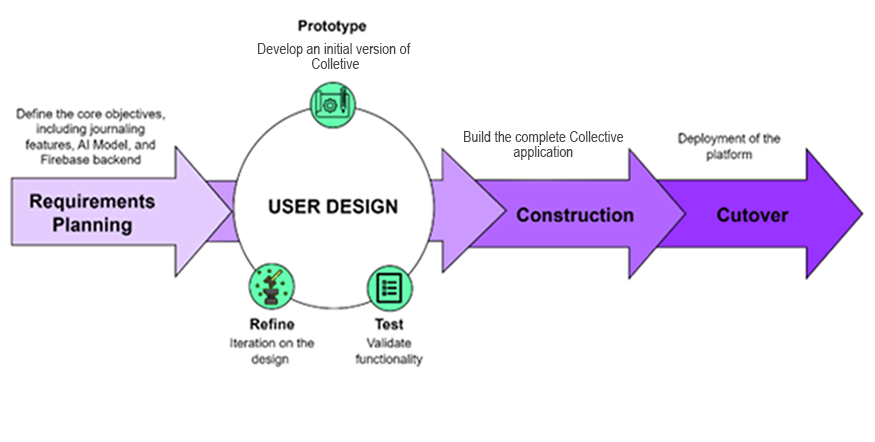
\includegraphics[width=0.8\textwidth]{files/imgs/RAD.png}
\caption{Rapid Application Development (RAD) Methodology Phases}
\label{fig:rad-methodology}
\end{figure}

Rapid Application Development (RAD) is a software development methodology that emphasizes quick development and iteration of prototypes over rigorous planning and testing. It is particularly useful for projects where requirements are expected to evolve or are not fully understood at the outset. The RAD methodology consists of four main phases: requirement planning, user design, construction, and cutover. This model was chosen for the development of the \textbf{Collective} mobile journaling application due to its flexibility and focus on user feedback, which is crucial for creating a user-friendly and effective application. The detais of the project is discussed below:

\section{Requirement planning}\label{sec:requirementPlanning}   

The requirement planning phase is the first step in the RAD methodology, where the project team identifies and defines the requirements of the application. This phase involves gathering information from stakeholders, including potential users, to understand their needs and expectations. The goal is to create a clear and concise set of requirements that will guide the development process.

\subsection{Software Requirements}\label{subsec:softwareRequirements}

The following tables list the software and tools used to develop the \textbf{Collective} mobile journaling application:

\begin{table}[H]
\centering
\caption{Visual Studio Code}
\label{tab:vscode-metadata}
\begin{tabular}{|p{4cm}|p{10cm}|}
\hline
\textbf{Attribute} & \textbf{Details} \\
\hline
Name & Visual Studio Code \\
\hline
Mnemonic & VS Code \\
\hline
Specification Number & N/A \\
\hline
Version Number & 1.101.1 \\
\hline
Source & \url{https://code.visualstudio.com/} \\
\hline
\end{tabular}
\end{table}

\begin{table}[H]
\centering
\caption{Flutter}
\label{tab:flutter-metadata}
\begin{tabular}{|p{4cm}|p{10cm}|}
\hline
\textbf{Attribute} & \textbf{Details} \\
\hline
Name & Flutter \\
\hline
Mnemonic & Flutter SDK \\
\hline
Specification Number & N/A \\
\hline
Version Number & 3.10.0 \\
\hline
Source & \url{https://flutter.dev/} \\
\hline
\end{tabular}
\end{table}

\begin{table}[H]
\centering
\caption{Dart}
\label{tab:dart-metadata}
\begin{tabular}{|p{4cm}|p{10cm}|}
\hline
\textbf{Attribute} & \textbf{Details} \\
\hline
Name & Dart \\
\hline
Mnemonic & Dart SDK \\
\hline
Specification Number & N/A \\
\hline
Version Number & 3.0.0 \\
\hline
Source & \url{https://dart.dev/} \\
\hline
\end{tabular}
\end{table}

\begin{table}[H]
\centering
\caption{Google Chrome}
\label{tab:chrome-metadata}
\begin{tabular}{|p{4cm}|p{10cm}|}
\hline
\textbf{Attribute} & \textbf{Details} \\
\hline
Name & Google Chrome \\
\hline
Mnemonic & Chrome Browser \\
\hline
Specification Number & N/A \\
\hline
Version Number & 114.0.5735.199 \\
\hline
Source & \url{https://www.google.com/chrome/} \\
\hline
\end{tabular}
\end{table}

\begin{table}[H]
\centering
\caption{Microsoft Word}
\label{tab:msword-metadata}
\begin{tabular}{|p{4cm}|p{10cm}|}
\hline
\textbf{Attribute} & \textbf{Details} \\
\hline
Name & Microsoft Word \\
\hline
Mnemonic & MS Word \\
\hline
Specification Number & N/A \\
\hline
Version Number & Office 365 \\
\hline
Source & \url{https://www.microsoft.com/en-us/microsoft-365/word} \\
\hline
\end{tabular}
\end{table}

\begin{table}[H]
\centering
\caption{Microsoft Excel}
\label{tab:msexcel-metadata}
\begin{tabular}{|p{4cm}|p{10cm}|}
\hline
\textbf{Attribute} & \textbf{Details} \\
\hline
Name & Microsoft Excel \\
\hline
Mnemonic & MS Excel \\
\hline
Specification Number & N/A \\
\hline
Version Number & Office 365 \\
\hline
Source & \url{https://www.microsoft.com/en-us/microsoft-365/excel} \\
\hline
\end{tabular}
\end{table}

\begin{table}[H]
\centering
\caption{Draw.io}
\label{tab:drawio-metadata}
\begin{tabular}{|p{4cm}|p{10cm}|}
\hline
\textbf{Attribute} & \textbf{Details} \\
\hline
Name & Draw.io \\
\hline
Mnemonic & Diagram Tool \\
\hline
Specification Number & N/A \\
\hline
Version Number & 20.8.0 \\
\hline
Source & \url{https://app.diagrams.net/} \\
\hline
\end{tabular}
\end{table}

\begin{table}[H]
\centering
\caption{DeepSeek API}
\label{tab:deepseek-metadata}
\begin{tabular}{|p{4cm}|p{10cm}|}
\hline
\textbf{Attribute} & \textbf{Details} \\
\hline
Name & DeepSeek API \\
\hline
Mnemonic & DeepSeek \\
\hline
Specification Number & N/A \\
\hline
Version Number & DeepSeek-V3-0324 \\
\hline
Source & \url{https://platform.deepseek.com/} \\
\hline
\end{tabular}
\end{table}

\subsection{Hardware Requirements}\label{subsec:hardwareRequirements}

The following table lists the hardware requirements necessary for the development and testing of the \textbf{Collective} mobile journaling application. Note that the development is currently focused exclusively on the Android platform, as iOS development requires a macOS machine, which is planned for future work:

\begin{table}[H]
\centering
\caption{Hardware Requirements}
\label{tab:hardware-requirements}
\begin{tabular}{|p{4cm}|p{10cm}|}
\hline
\textbf{Component} & \textbf{Specification} \\
\hline
Processor & Intel Core i5 or equivalent \\
\hline
RAM & 8 GB or higher \\
\hline
Storage & 256 GB SSD or higher \\
\hline
Operating System & Windows 10 \\
\hline
Additional Devices & Android smartphone for testing \\
\hline
\end{tabular}
\end{table}

\subsection{Use Case Diagram}\label{subsec:usecaseDiagram}

The use case diagram for the \textbf{Collective} mobile journaling application illustrates the interactions between the user (Writer) and the system. It highlights the various functionalities provided by the application and their relationships. The diagram is shown below:

\begin{figure}[H]
\centering
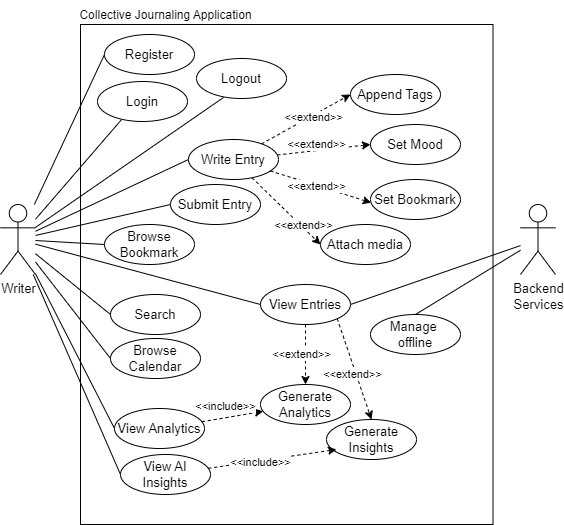
\includegraphics[width=0.8\textwidth]{files/imgs/usecase_diagram.png}
\caption{Use Case Diagram for Collective Mobile Journaling Application}
\label{fig:usecase-diagram}
\end{figure}

\subsection{Use Case Description}\label{subsec:usecaseDescription}

The use case description provides detailed information about the functionalities depicted in the use case diagram. Below is a table summarizing the key use cases:

\begin{table}[H]
\centering
\caption{Use Case Description}
\label{tab:usecase-description}
\begin{tabular}{|p{3cm}|p{5cm}|p{7cm}|}
\hline
\textbf{Actor} & \textbf{Use Case} & \textbf{Use Case Description} \\
\hline
\multirow{15}{*}{Writer} & Register & The writer can register their account by filling in their name, email, and password or use X or Google to register. \\
\cline{2-3}
 & Login & The writer can log in to the application using their registered credentials. \\
\cline{2-3}
 & Logout & The writer can log out of the application when they are done. \\
\cline{2-3}
 & Write Entry & The writer can compose journal entries to record their thoughts and experiences. \\
\cline{2-3}
 & Append Tags & The writer can add tags to their journal entries for better organization. \\
\cline{2-3}
 & Set Mood & The writer can set their mood for each journal entry to reflect their feelings. \\
\cline{2-3}
 & Set Bookmark & The writer can bookmark specific entries for quick access later. \\
\cline{2-3}
 & Attach Media & The writer can attach images or other media to their journal entries. \\
\cline{2-3}
 & Submit Entry & The writer can submit their journal entries to save them in the application. \\
\cline{2-3}
 & Browse Bookmark & The writer can browse through their bookmarked entries. \\
\cline{2-3}
 & View Entries & The writer can view all their saved journal entries. \\
\cline{2-3}
 & Search & The writer can search for specific entries using keywords. \\
\cline{2-3}
 & Browse Calendar & The writer can view their journal entries organized by calendar dates. \\
\cline{2-3}
 & View Analytics & The writer can analyze their journal entries to gain insights into their habits and patterns. \\
\cline{2-3}
 & View AI Insights & The writer can access AI-generated insights based on their journal entries. \\
\hline
\multirow{4}{*}{Backend Services} & View Entries & The system to store and retrieve the writer's journal entries securely. \\
\cline{2-3}
 & Manage Offline & The system to allow the writer to access their entries even when offline. \\
\cline{2-3}
 & Generate Analytics & The system to analyze the writer's journal entries to provide useful statistics. \\
\cline{2-3}
 & Generate Insights & The system to generate insights based on the writer's journal entries to help them understand their patterns. \\
\hline
\end{tabular}
\end{table}

\section{User design}\label{sec:userDesign}

The user design phase focuses on how users interact with the Collective application, shaping the interface and workflow based on user feedback and usability principles. This section details the main user roles and their interactions with the system, illustrated with activity diagrams for each core function.

% 3.4.1 Writer
\subsection{Writer}\label{subsec:writer}

The Writer is the primary user of the Collective application, responsible for creating, managing, and analyzing journal entries. The following functions are available to the Writer:

\textbf{i. Register}

Figure~\ref{fig:register-flow} shows the registration flow for new users. The writer can register using their email and password or authenticate through Google/X OAuth providers. The system validates the account details and, upon successful registration, redirects the writer to the journal screen where they can begin their journaling experience.

\begin{figure}[H]
\centering
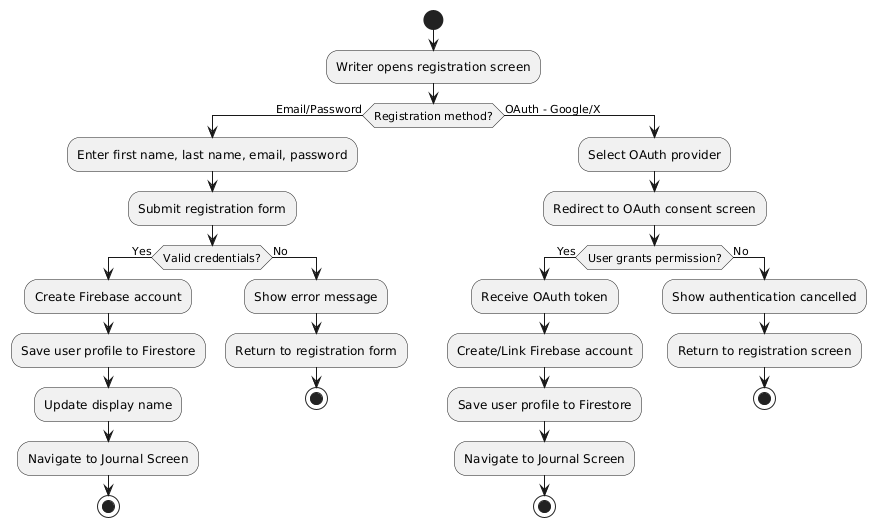
\includegraphics[width=0.8\textwidth]{files/imgs/register_flow.png}
\caption{Registration flow for Writer}
\label{fig:register-flow}
\end{figure}

\textbf{ii. Login}

Figure~\ref{fig:login-flow} shows the login flow for existing users. The writer can authenticate using their registered email and password or through their previously linked Google/X account. Upon successful authentication, the system validates the credentials and redirects the writer to the main journal screen.

\begin{figure}[H]
\centering
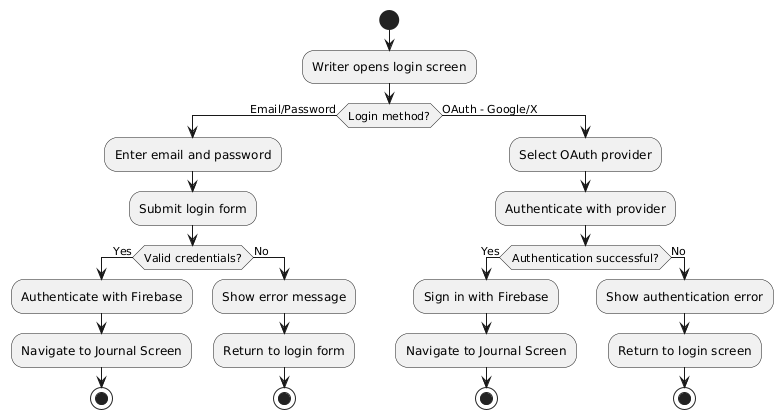
\includegraphics[width=0.8\textwidth]{files/imgs/login_flow.png}
\caption{Login flow for Writer}
\label{fig:login-flow}
\end{figure}

\textbf{iii. Write Entry}

Figure~\ref{fig:write-entry-flow} shows the entry creation flow for writers. The writer composes their journal entry in a distraction-free interface, optionally adds mood, tags, and media attachments, then saves the entry using the prominently displayed save button. The system processes the entry both locally and in the cloud when connectivity is available.

\begin{figure}[H]
\centering
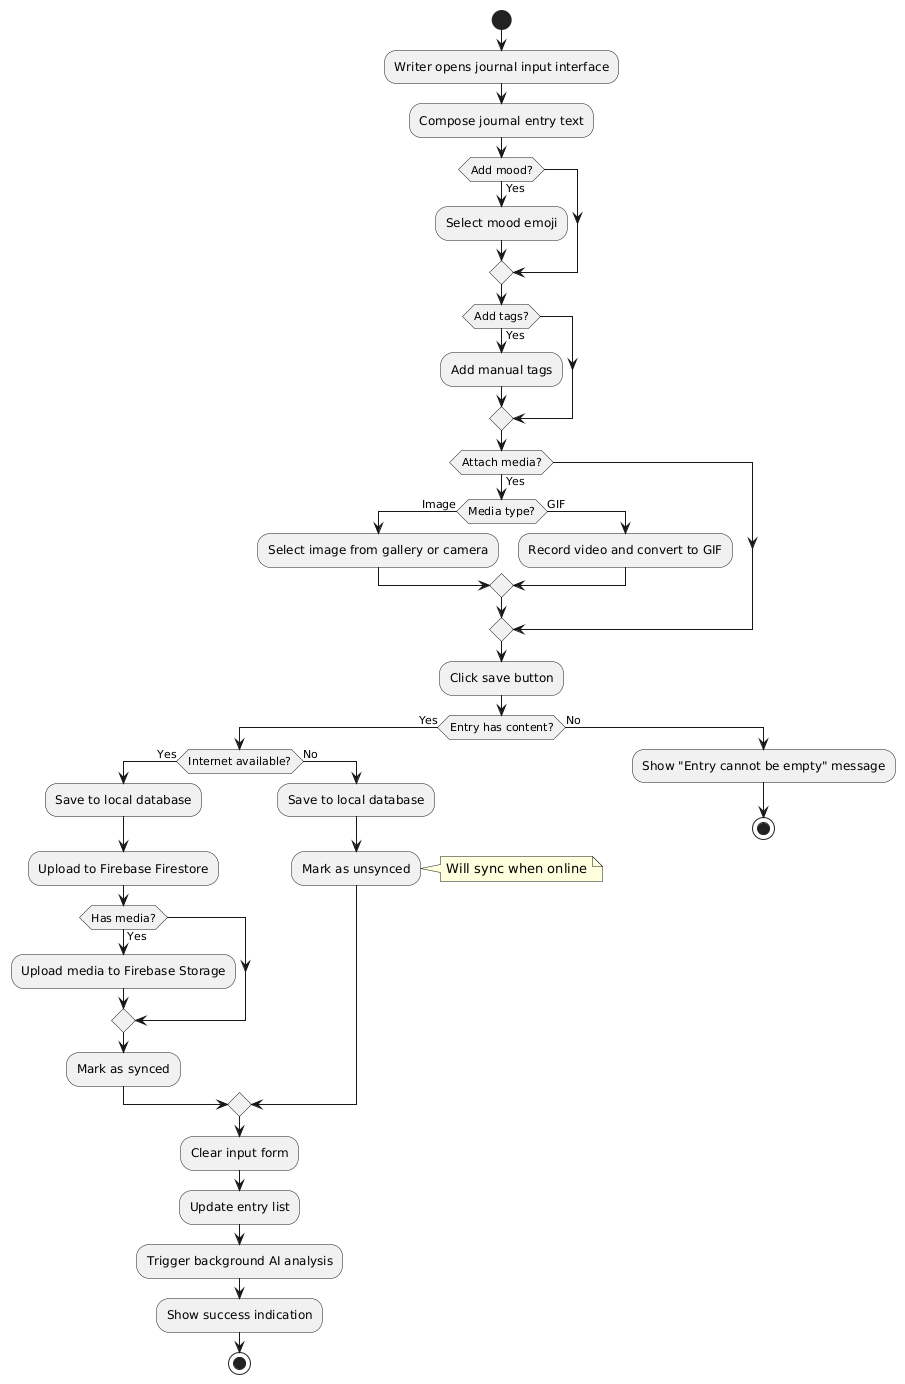
\includegraphics[width=0.8\textwidth]{files/imgs/write_entry_flow.png}
\caption{Write Entry flow for Writer}
\label{fig:write-entry-flow}
\end{figure}

\textbf{iv. Edit Entry}

Figure~\ref{fig:edit-entry-flow} shows the entry editing flow for writers. The writer can modify existing entries, update their mood, change tags, or replace media attachments. The system tracks changes and updates both local and cloud storage accordingly.

\begin{figure}[H]
\centering
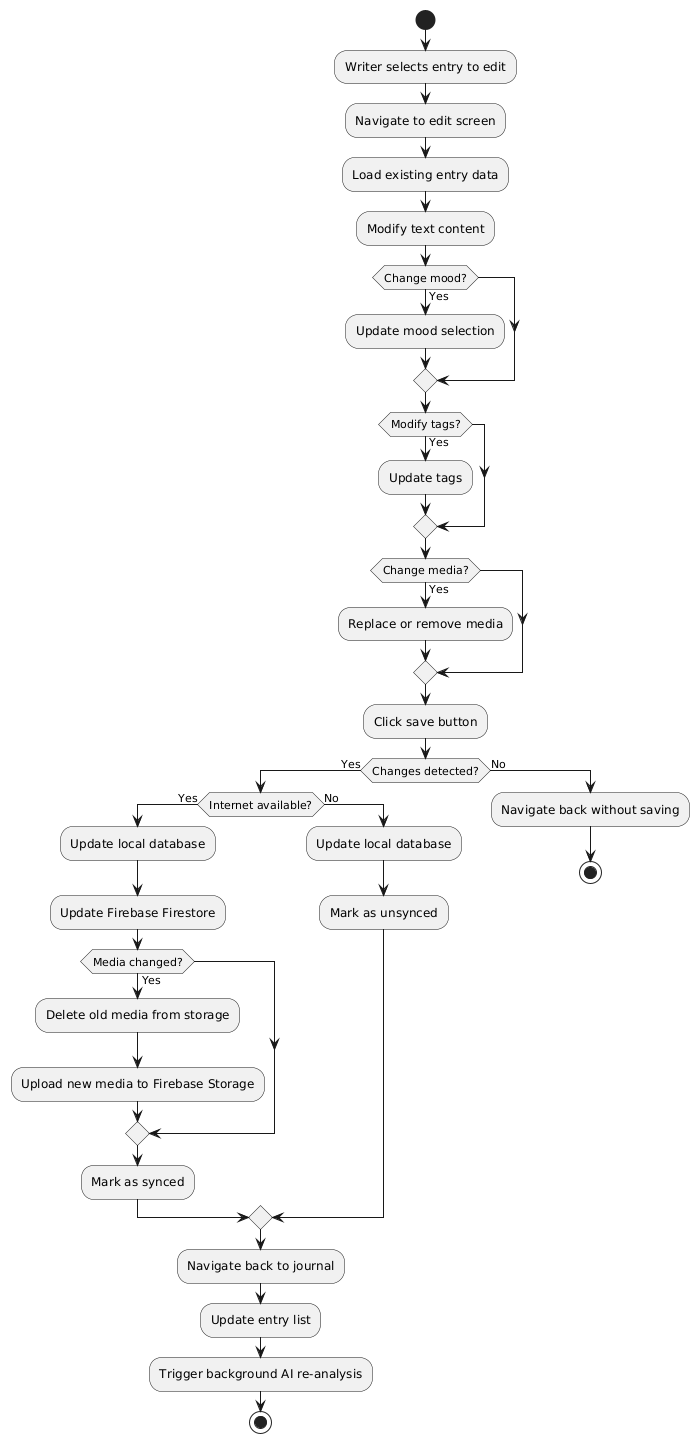
\includegraphics[width=0.8\textwidth]{files/imgs/edit_entry_flow.png}
\caption{Edit Entry flow for Writer}
\label{fig:edit-entry-flow}
\end{figure}

\textbf{v. Search}

Figure~\ref{fig:search-flow} shows the search functionality flow. The writer can search through their entries using fuzzy search algorithms that match both entry content and tags, providing intelligent search results even with partial or approximate queries.

\begin{figure}[H]
\centering
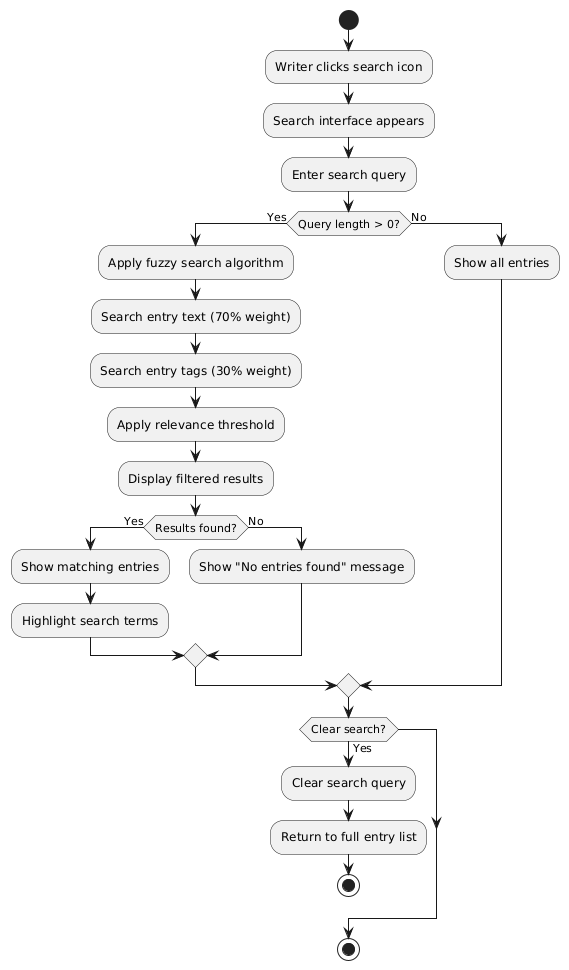
\includegraphics[width=0.8\textwidth]{files/imgs/search_flow.png}
\caption{Search flow for Writer}
\label{fig:search-flow}
\end{figure}

\textbf{vi. Analytics}

Figure~\ref{fig:analytics-flow} shows the analytics viewing flow. The writer can access AI-generated insights about their journaling patterns, emotional trends, and topic clusters. The system uses cached analytics data when available and generates new analysis when needed.

\begin{figure}[H]
\centering
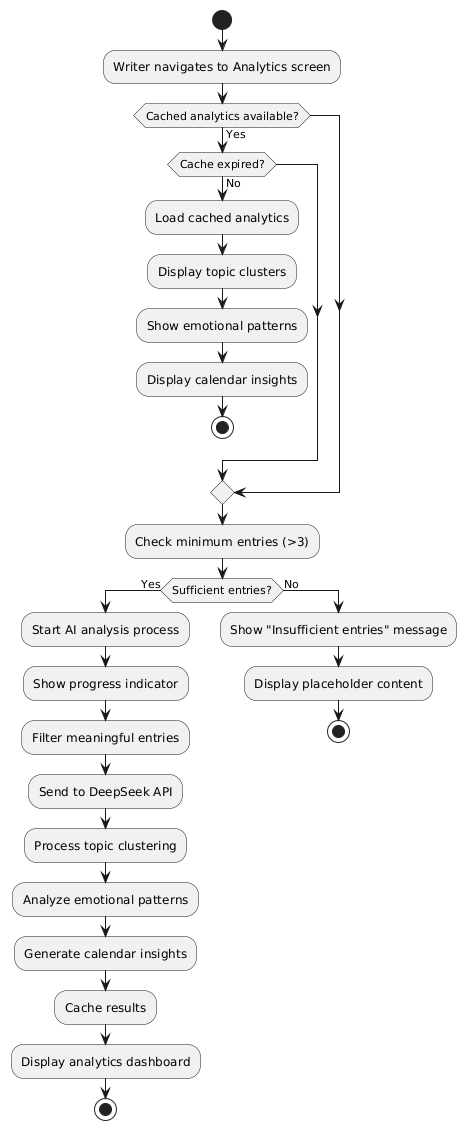
\includegraphics[width=0.8\textwidth]{files/imgs/analytics_flow.png}
\caption{Analytics flow for Writer}
\label{fig:analytics-flow}
\end{figure}

\textbf{vii. Insights}

Figure~\ref{fig:insights-flow} shows the AI insights viewing flow for individual entries. The writer can access detailed analysis of specific entries, including contextual relationships, emotional analysis, and personalized recommendations.

\begin{figure}[H]
\centering
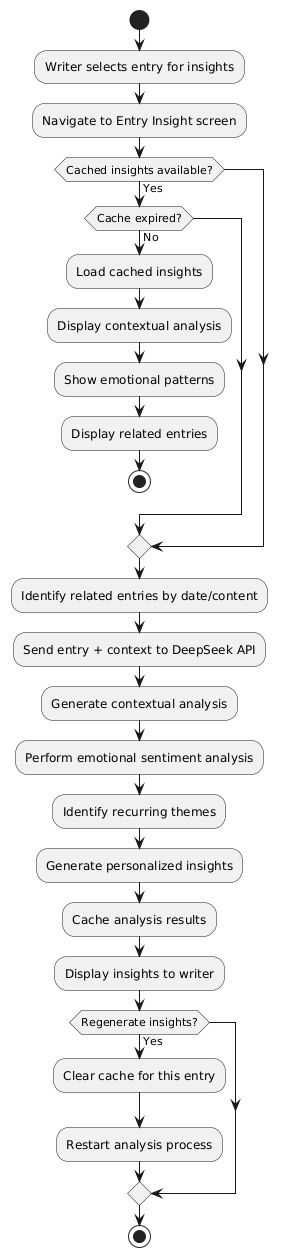
\includegraphics[width=0.8\textwidth]{files/imgs/insights_flow.png}
\caption{Insights flow for Writer}
\label{fig:insights-flow}
\end{figure}

\textbf{viii. Logout}

Figure~\ref{fig:logout-flow} shows the logout process for writers. The system securely terminates the user session, clears authentication tokens, and redirects to the login screen while ensuring local data remains protected.

\begin{figure}[H]
\centering
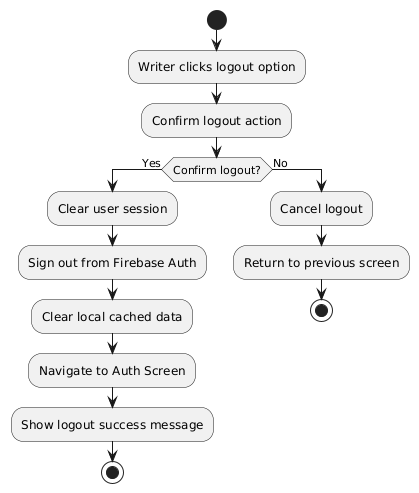
\includegraphics[width=0.8\textwidth]{files/imgs/logout_flow.png}
\caption{Logout flow for Writer}
\label{fig:logout-flow}
\end{figure}

\textbf{ix. Append Tags}

Figure~\ref{fig:append-tags-flow} shows the tag management flow. Writers can add, modify, or remove tags from their entries to improve organization and searchability. The system provides tag suggestions based on entry content and previous usage patterns.

\begin{figure}[H]
\centering
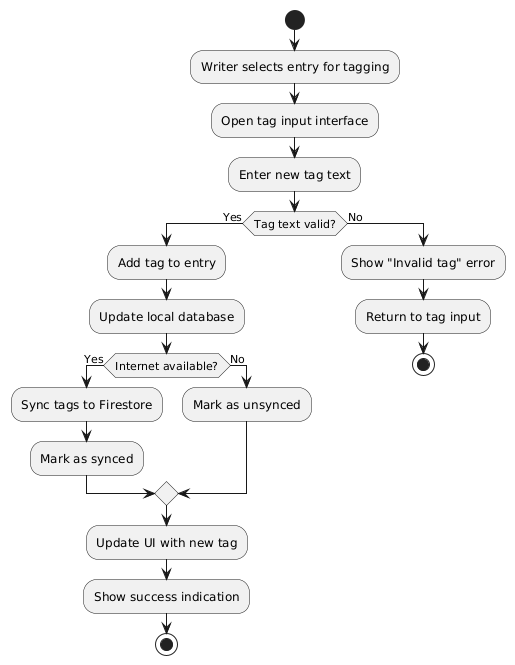
\includegraphics[width=0.8\textwidth]{files/imgs/append_tags_flow.png}
\caption{Append Tags flow for Writer}
\label{fig:append-tags-flow}
\end{figure}

\textbf{x. Set Mood}

Figure~\ref{fig:set-mood-flow} shows the mood setting functionality. Writers can associate emotional states with their entries, enabling the system to track emotional patterns over time and provide relevant insights.

\begin{figure}[H]
\centering
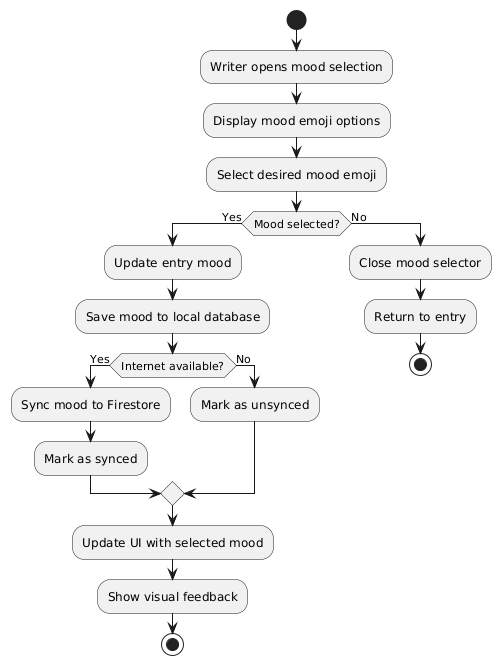
\includegraphics[width=0.8\textwidth]{files/imgs/set_mood_flow.png}
\caption{Set Mood flow for Writer}
\label{fig:set-mood-flow}
\end{figure}

\textbf{xi. Set Bookmark}

Figure~\ref{fig:set-bookmark-flow} shows the bookmarking process. Writers can mark important entries for quick access, creating a personalized collection of significant journal entries.

\begin{figure}[H]
\centering
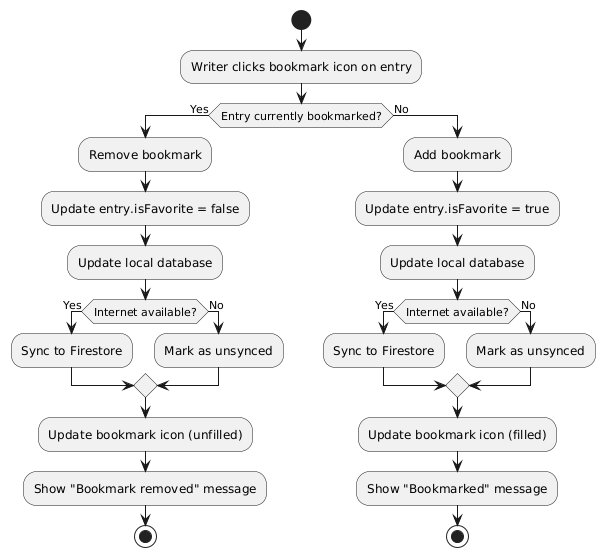
\includegraphics[width=0.8\textwidth]{files/imgs/set_bookmark_flow.png}
\caption{Set Bookmark flow for Writer}
\label{fig:set-bookmark-flow}
\end{figure}

\textbf{xii. Attach Media}

Figure~\ref{fig:attach-media-flow} shows the media attachment process. Writers can enhance their entries with images, GIFs, or other media content, with the system handling compression and storage optimization automatically.

\begin{figure}[H]
\centering
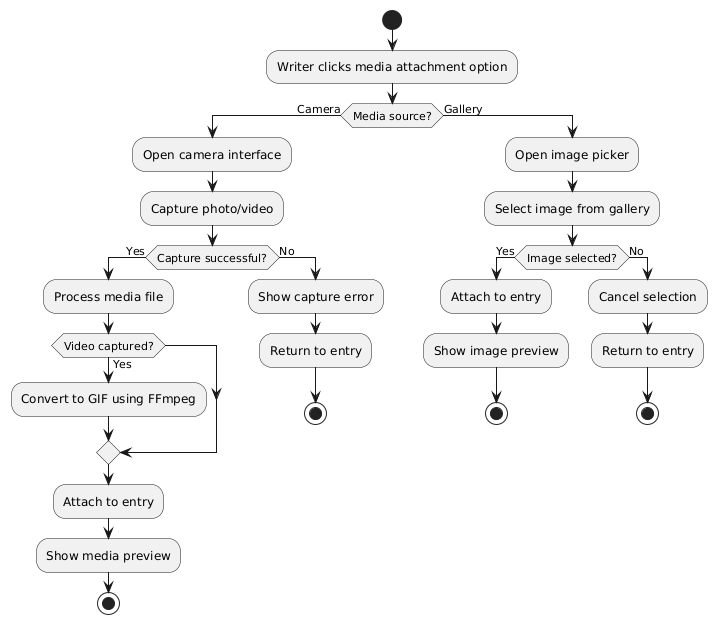
\includegraphics[width=0.8\textwidth]{files/imgs/attach_media_flow.png}
\caption{Attach Media flow for Writer}
\label{fig:attach-media-flow}
\end{figure}

\textbf{xiii. Browse Bookmark}

Figure~\ref{fig:browse-bookmark-flow} shows the bookmark browsing functionality. Writers can efficiently navigate through their bookmarked entries, with options for sorting and filtering based on various criteria.

\begin{figure}[H]
\centering
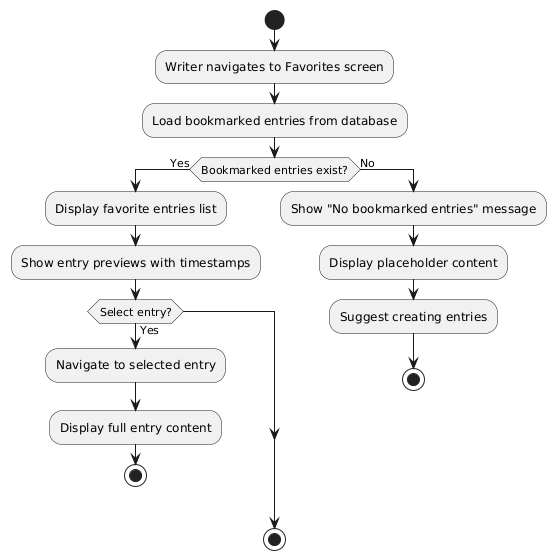
\includegraphics[width=0.8\textwidth]{files/imgs/browse_bookmark_flow.png}
\caption{Browse Bookmark flow for Writer}
\label{fig:browse-bookmark-flow}
\end{figure}

\textbf{xiv. View Entries}

Figure~\ref{fig:view-entries-flow} shows the entry viewing interface. Writers can browse through all their journal entries with various viewing options including list view, timeline view, and calendar integration.

\begin{figure}[H]
\centering
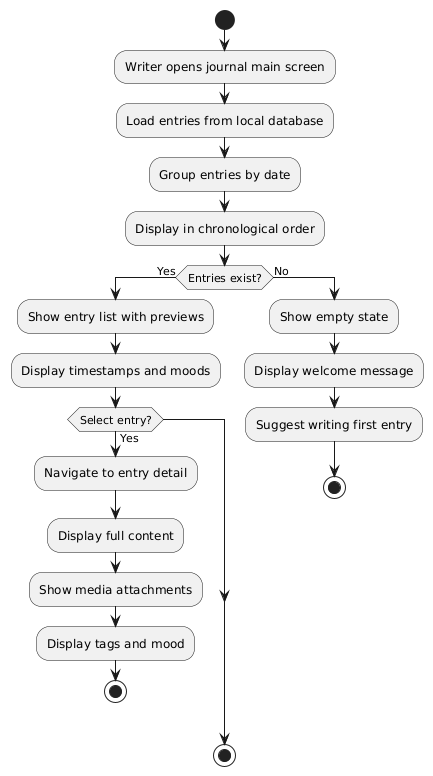
\includegraphics[width=0.8\textwidth]{files/imgs/view_entries_flow.png}
\caption{View Entries flow for Writer}
\label{fig:view-entries-flow}
\end{figure}

\textbf{xv. Browse Calendar}

Figure~\ref{fig:browse-calendar-flow} shows the calendar browsing functionality. Writers can navigate through their journaling history using an intuitive calendar interface, quickly jumping to entries from specific dates.

\begin{figure}[H]
\centering
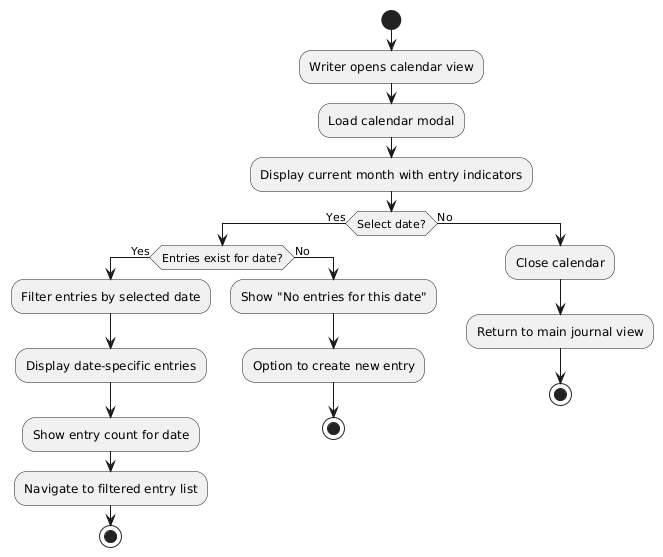
\includegraphics[width=0.8\textwidth]{files/imgs/browse_calendar_flow.png}
\caption{Browse Calendar flow for Writer}
\label{fig:browse-calendar-flow}
\end{figure}

% 3.4.2 Backend Services
\subsection{Backend Services}\label{subsec:backendServices}

This subsection covers the backend functionalities that support the user-facing features, including data management, synchronization, and AI processing capabilities.

\subsubsection{Store/Retrieve Entries}\label{subsubsec:storeRetrieveEntries}

Figure \ref{fig:store-retrieve-entries-flow} shows the data management process for journal entries. The system handles secure storage and retrieval of entries across local and cloud storage, ensuring data integrity and availability.

\begin{figure}[H]
\centering
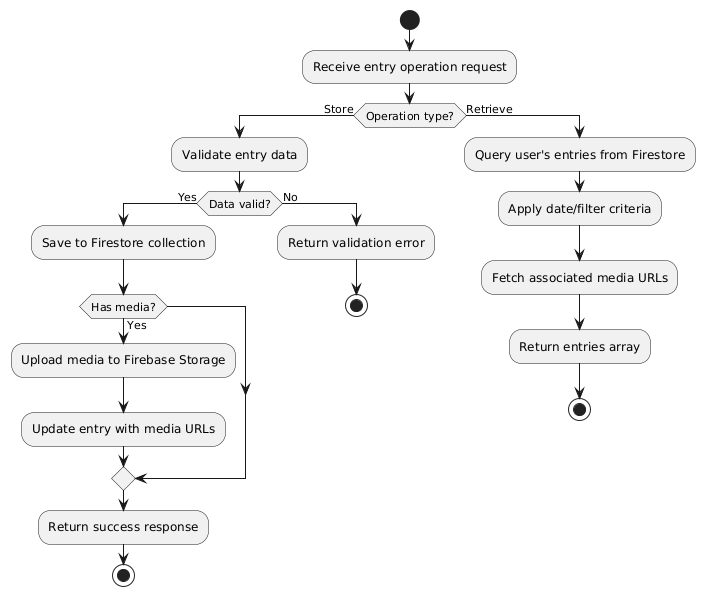
\includegraphics[width=0.8\textwidth]{files/imgs/store_retrieve_entries_flow.png}
\caption{Store/Retrieve Entries Flow}
\label{fig:store-retrieve-entries-flow}
\end{figure}

\subsubsection{Manage Offline}\label{subsubsec:manageOffline}

Figure \ref{fig:manage-offline-flow} shows the offline functionality management. The system automatically handles offline mode, local data storage, and synchronization when connectivity is restored, ensuring seamless user experience regardless of network availability.

\begin{figure}[H]
\centering
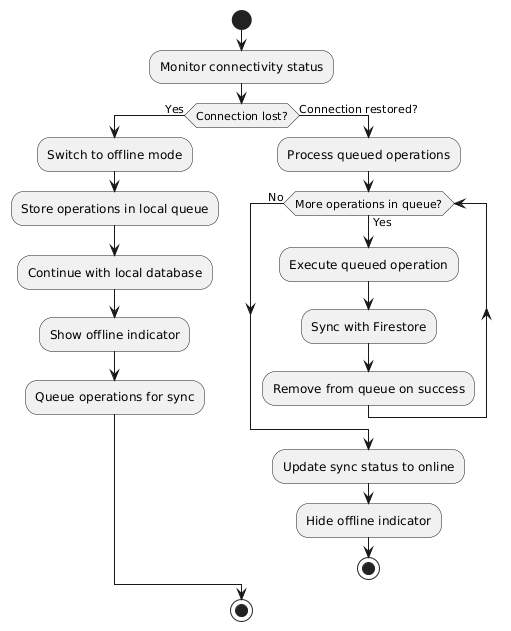
\includegraphics[width=0.8\textwidth]{files/imgs/manage_offline_flow.png}
\caption{Manage Offline Flow}
\label{fig:manage-offline-flow}
\end{figure}

\subsubsection{Sync}\label{subsubsec:sync}

Figure \ref{fig:sync-flow} shows the synchronization process between local and cloud storage. The system automatically detects connectivity changes and synchronizes data when internet access is available, maintaining data consistency across devices.

\begin{figure}[H]
\centering
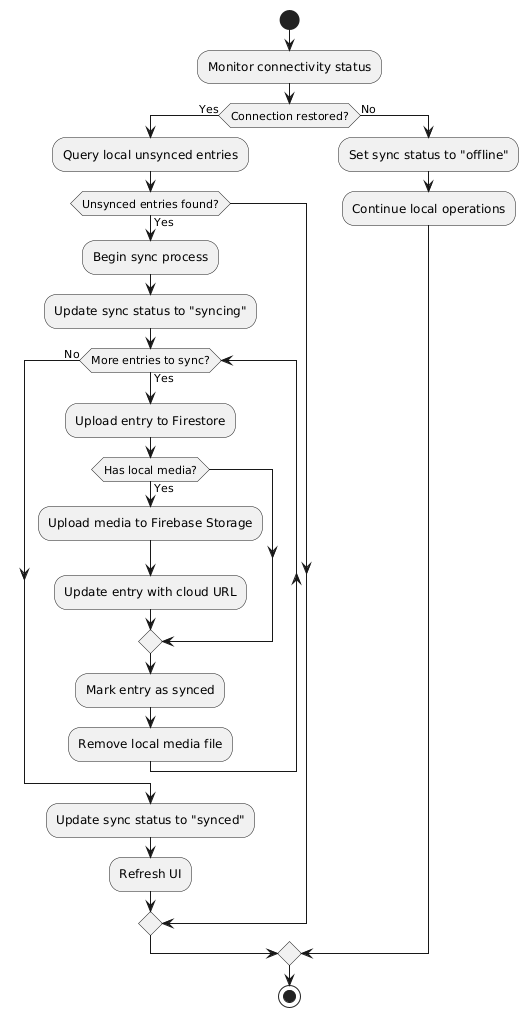
\includegraphics[width=0.8\textwidth]{files/imgs/sync_flow.png}
\caption{Synchronization Flow}
\label{fig:sync-flow}
\end{figure}

\subsubsection{AI Processing}\label{subsubsec:aiProcessing}

Figure \ref{fig:ai-processing-flow} shows the background AI processing that occurs automatically after entries are saved. The system performs sentiment analysis, pattern recognition, and insight generation without user intervention to maintain the simplicity of the journaling experience.

\begin{figure}[H]
\centering
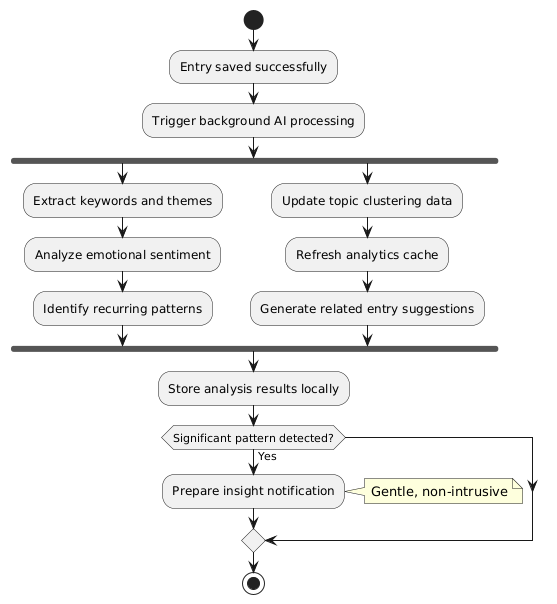
\includegraphics[width=0.8\textwidth]{files/imgs/ai_processing_flow.png}
\caption{AI Processing Flow}
\label{fig:ai-processing-flow}
\end{figure}

\section{Construction}\label{sec:construction}

The construction phase is the third phase of the RAD methodology where the actual development of the \textbf{Collective} mobile journaling application takes place. This phase involves implementing the designs and specifications defined in the user design phase. The development follows an iterative approach with continuous testing and refinement based on user feedback and technical requirements.

\subsection{Development Approach}\label{subsec:developmentApproach}

The construction phase employs an agile development approach with the following key characteristics:

\begin{enumerate}
    \item \textbf{Iterative Development}: Features are developed in small, manageable iterations allowing for quick feedback and adjustments.
    
    \item \textbf{Component-Based Architecture}: The application is built using modular components that can be developed and tested independently.
    
    \item \textbf{Continuous Integration}: Regular integration of code changes ensures that the application remains stable throughout development.
    
    \item \textbf{User Feedback Integration}: Regular user testing sessions inform development decisions and feature refinements.
\end{enumerate}

\subsection{Technical Implementation}\label{subsec:technicalImplementation}

The technical implementation follows the architecture designed in the user design phase:

\begin{enumerate}
    \item \textbf{Frontend Development}: Flutter framework is used to create a cross-platform mobile application with a focus on Android deployment.
    
    \item \textbf{Backend Integration}: Firebase services are integrated for authentication, data storage, and file management.
    
    \item \textbf{AI Integration}: DeepSeek API is integrated for natural language processing and intelligent analysis features.
    
    \item \textbf{Local Storage}: Sembast database is implemented for offline functionality and data synchronization.
    
    \item \textbf{Media Processing}: Camera integration and FFmpeg are used for image and GIF processing capabilities.
\end{enumerate}

\subsection{Quality Assurance}\label{subsec:qualityAssurance}

Throughout the construction phase, quality assurance measures are implemented:

\begin{enumerate}
    \item \textbf{Unit Testing}: Individual components are tested to ensure functionality.
    
    \item \textbf{Integration Testing}: Component interactions are tested to verify system integration.
    
    \item \textbf{User Acceptance Testing}: Regular testing with target users to validate user experience.
    
    \item \textbf{Performance Testing}: Application performance is monitored and optimized for mobile devices.
\end{enumerate}

\section{Cutover}\label{sec:cutover}

The cutover phase is the final phase of the RAD methodology where the \textbf{Collective} mobile journaling application is prepared for deployment and made available to end users. This phase involves final testing, deployment preparation, and the transition from development to production environment.

\subsection{Pre-Deployment Activities}\label{subsec:preDeployment}

Before the application is released, several critical activities are completed:

\begin{enumerate}
    \item \textbf{Final System Testing}: Comprehensive testing of all features and functionalities to ensure system stability.
    
    \item \textbf{Security Review}: Security assessment of authentication, data storage, and API integrations.
    
    \item \textbf{Performance Optimization}: Final performance tuning to ensure optimal user experience on target devices.
    
    \item \textbf{Documentation Completion}: User documentation and technical documentation are finalized.
\end{enumerate}

\subsection{Deployment Strategy}\label{subsec:deploymentStrategy}

The deployment strategy for Collective includes:

\begin{enumerate}
    \item \textbf{Platform Preparation}: Android APK is prepared for distribution through Google Play Store or direct installation.
    
    \item \textbf{Backend Configuration}: Firebase services are configured for production use with appropriate security settings.
    
    \item \textbf{API Configuration}: DeepSeek API integration is configured for production workloads.
    
    \item \textbf{Monitoring Setup}: Application monitoring and analytics are configured to track user engagement and system performance.
\end{enumerate}

\subsection{User Training and Support}\label{subsec:userSupport}

To ensure successful adoption of the application:

\begin{enumerate}
    \item \textbf{User Onboarding}: In-app tutorials and guidance are provided to help new users understand the application features.
    
    \item \textbf{Documentation}: User guides and frequently asked questions are made available.
    
    \item \textbf{Feedback Channels}: Mechanisms are established for users to provide feedback and report issues.
    
    \item \textbf{Continuous Improvement}: A process is established for collecting user feedback and implementing improvements.
\end{enumerate}

\subsection{Post-Deployment Activities}\label{subsec:postDeployment}

After the application is deployed, ongoing activities include:

\begin{enumerate}
    \item \textbf{User Monitoring}: Tracking user engagement and application usage patterns.
    
    \item \textbf{Performance Monitoring}: Monitoring application performance and system reliability.
    
    \item \textbf{Feature Enhancement}: Planning and implementing new features based on user feedback.
    
    \item \textbf{Maintenance}: Regular updates and bug fixes to maintain application quality.
\end{enumerate}

The successful completion of the cutover phase marks the transition of Collective from a development project to a production application ready for use by writers seeking an intelligent journaling experience.